\documentclass[11pt,a4paper]{report}
\usepackage[textwidth=37em,vmargin=30mm]{geometry}
\usepackage{calc,xunicode,amsmath,amssymb,paralist,enumitem,tabu,booktabs,datetime2,xeCJK,xeCJKfntef,listings}
\usepackage{tocloft,fancyhdr,tcolorbox,xcolor,graphicx,eso-pic,xltxtra,xelatexemoji}

\newcommand{\envyear}[0]{2024}
\newcommand{\envdatestr}[0]{2024-10-12}
\newcommand{\envfinaldir}[0]{webdb/2024/20241012/final}

\usepackage[hidelinks]{hyperref}
\hypersetup{
    colorlinks=false,
    pdfpagemode=FullScreen,
    pdftitle={Web Digest - \envdatestr}
}

\setlength{\cftbeforechapskip}{10pt}
\renewcommand{\cftchapfont}{\rmfamily\bfseries\large\raggedright}
\setlength{\cftbeforesecskip}{2pt}
\renewcommand{\cftsecfont}{\sffamily\small\raggedright}

\setdefaultleftmargin{2em}{2em}{1em}{1em}{1em}{1em}

\usepackage{xeCJK,xeCJKfntef}
\xeCJKsetup{PunctStyle=plain,RubberPunctSkip=false,CJKglue=\strut\hskip 0pt plus 0.1em minus 0.05em,CJKecglue=\strut\hskip 0.22em plus 0.2em}
\XeTeXlinebreaklocale "zh"
\XeTeXlinebreakskip = 0pt


\setmainfont{Brygada 1918}
\setromanfont{Brygada 1918}
\setsansfont{IBM Plex Sans}
\setmonofont{JetBrains Mono NL}
\setCJKmainfont{Noto Serif CJK SC}
\setCJKromanfont{Noto Serif CJK SC}
\setCJKsansfont{Noto Sans CJK SC}
\setCJKmonofont{Noto Sans CJK SC}

\setlength{\parindent}{0pt}
\setlength{\parskip}{8pt}
\linespread{1.15}

\lstset{
	basicstyle=\ttfamily\footnotesize,
	numbersep=5pt,
	backgroundcolor=\color{black!5},
	showspaces=false,
	showstringspaces=false,
	showtabs=false,
	tabsize=2,
	captionpos=b,
	breaklines=true,
	breakatwhitespace=true,
	breakautoindent=true,
	linewidth=\textwidth
}






\newcommand{\coverpic}[2]{
    % argv: itemurl, authorname
    Cover photo by #2~~(\href{#1}{#1})
}
\newcommand{\makeheader}[0]{
    \begin{titlepage}
        % \newgeometry{hmargin=15mm,tmargin=21mm,bmargin=12mm}
        \begin{center}
            
            \rmfamily\scshape
            \fontspec{BaskervilleF}
            \fontspec{Old Standard}
            \fontsize{59pt}{70pt}\selectfont
            WEB\hfill DIGEST
            
            \vfill
            % \vskip 30pt
            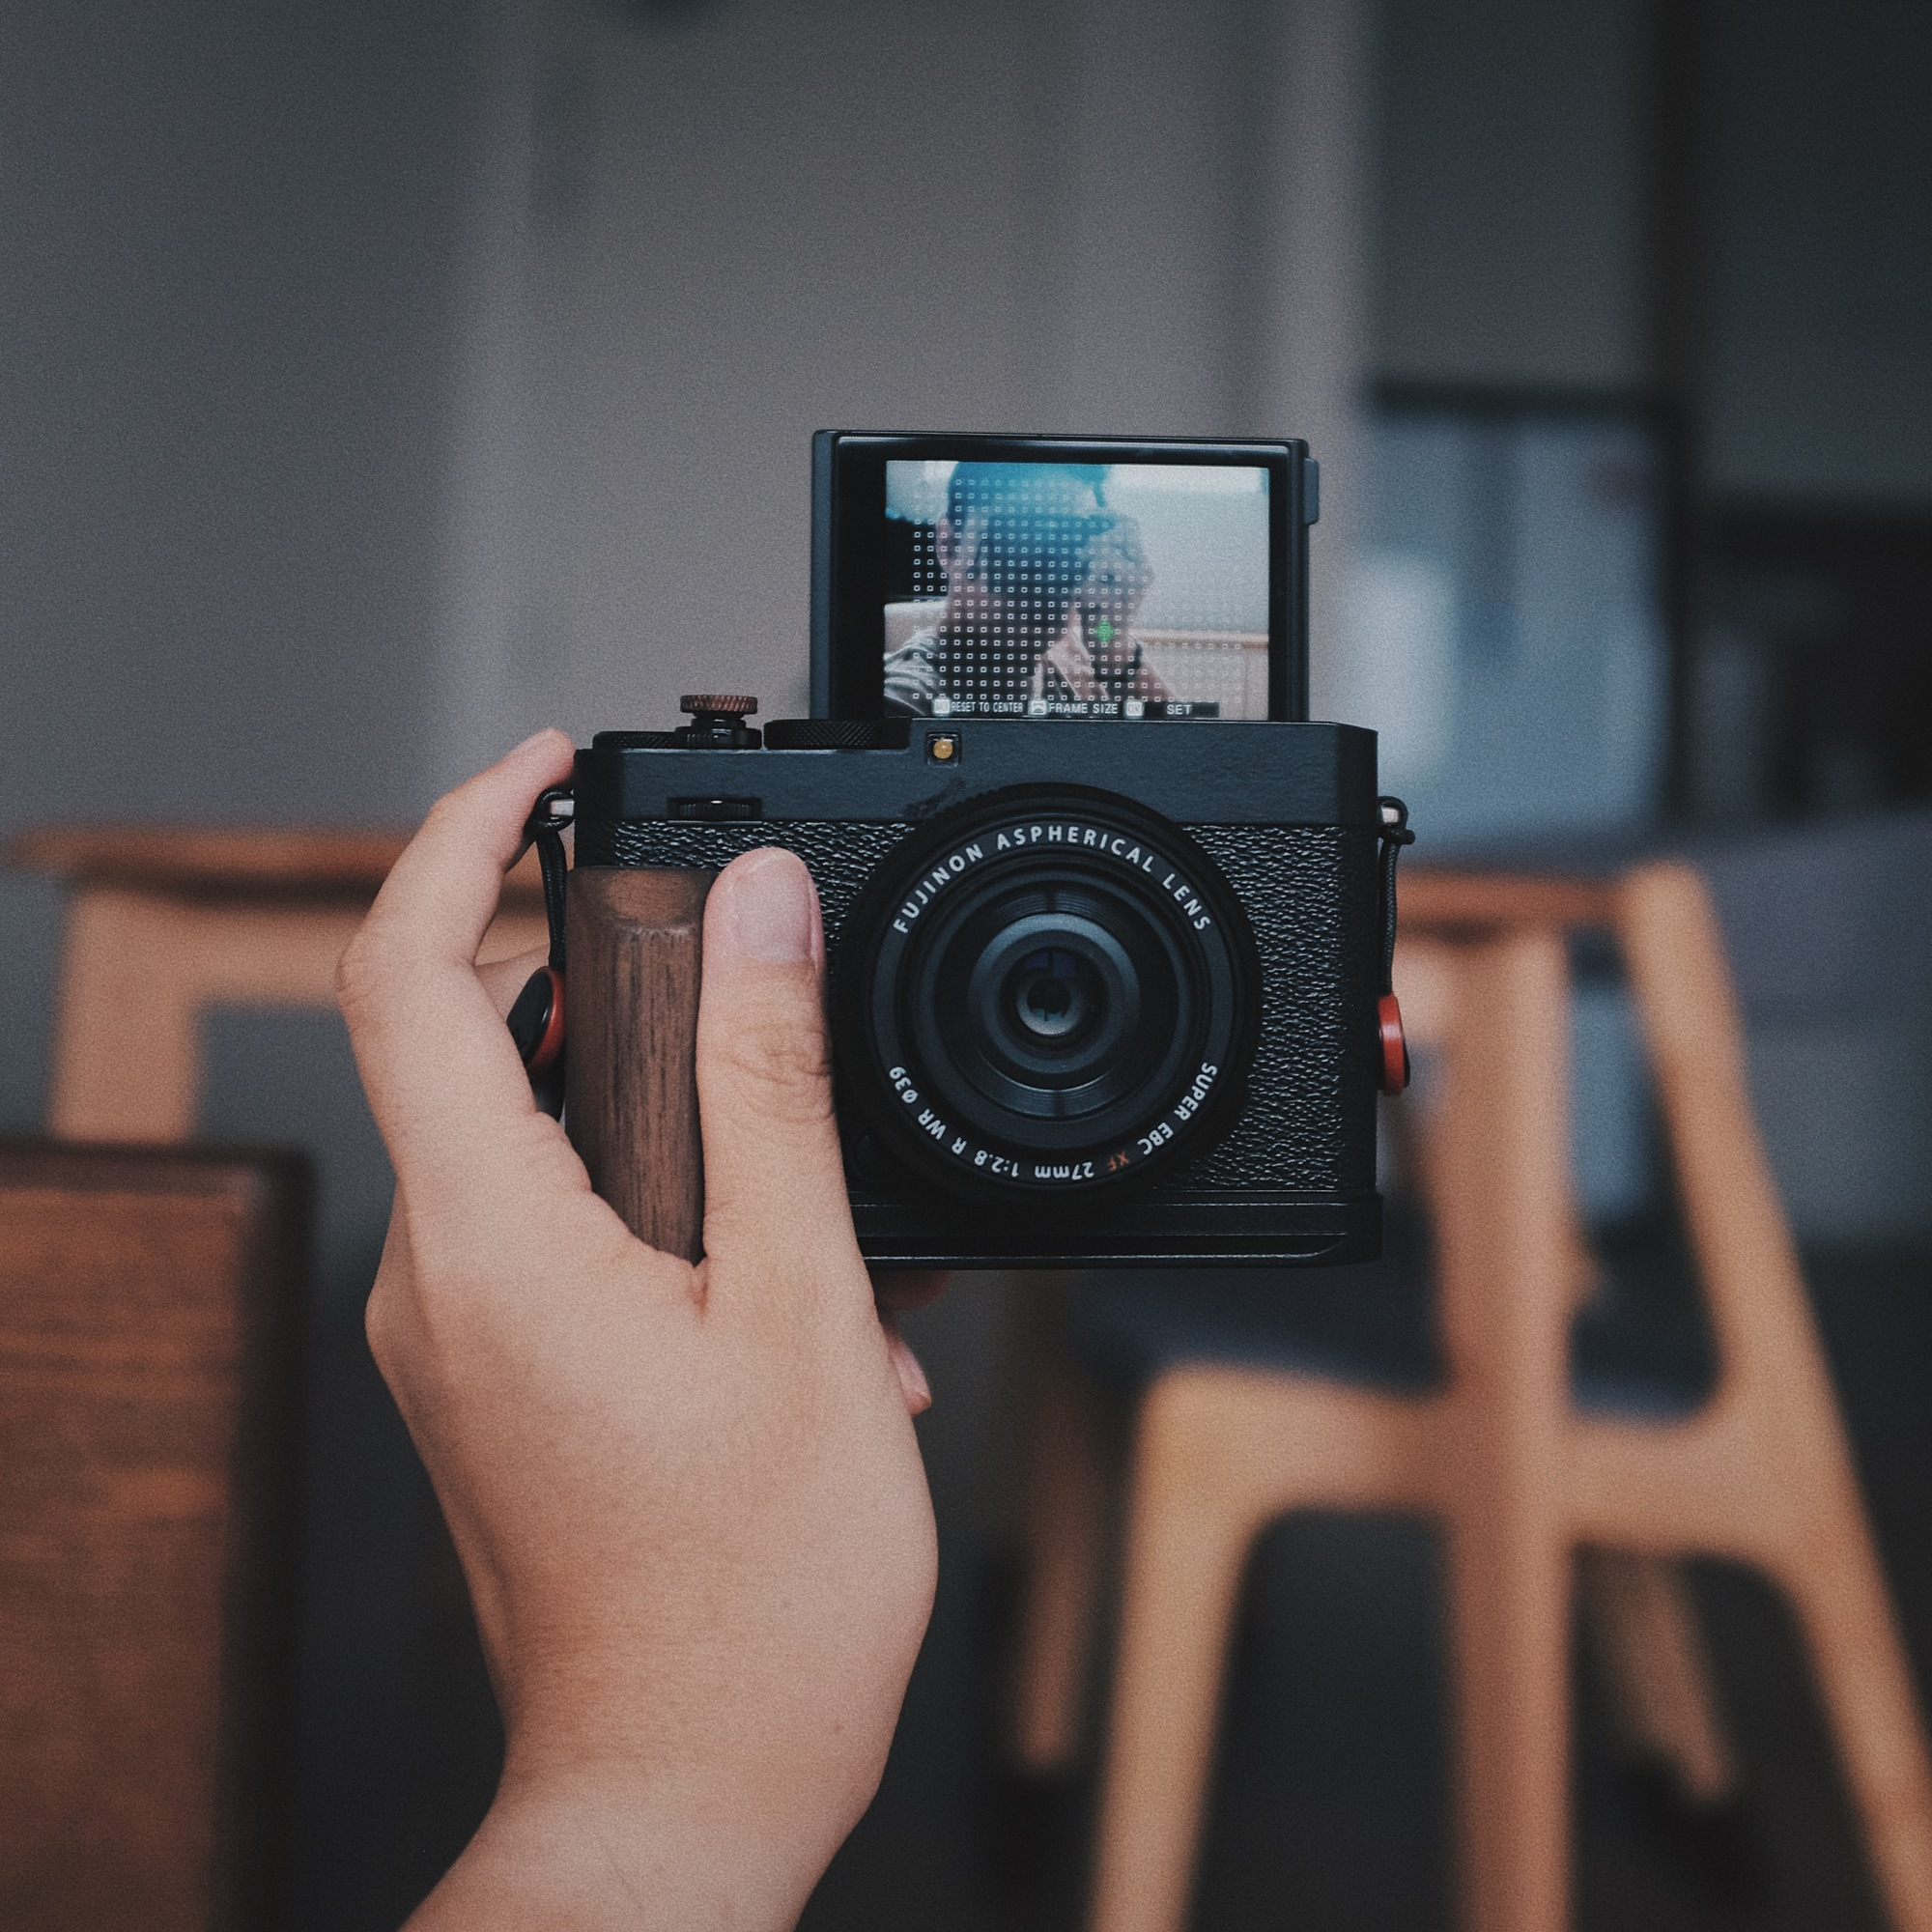
\includegraphics[width=\linewidth]{\envfinaldir/coverpic-prod.jpg}\par
            % \vskip 30pt
            \vfill

            \normalsize\rmfamily\scshape
            \copyright{} The Web Digest Project \hfill\large \envdatestr
        \end{center}
    \end{titlepage}
    % \restoregeometry
}
\newcommand{\simplehref}[1]{%
    \textcolor{blue!80!green}{\href{#1}{#1}}%
}
\renewcommand{\contentsname}{\center\Huge\sffamily\bfseries Contents\par\vskip 20pt}
\newcounter{ipartcounter}
\setcounter{ipartcounter}{0}
\newcommand{\ipart}[1]{
    % \vskip 20pt
    \clearpage
    \stepcounter{ipartcounter}
    \phantomsection
    \addcontentsline{toc}{chapter}{#1}
    % \begin{center}
    %     \Huge
    %     \sffamily\bfseries
    %     #1
    % \end{center}
    % \vskip 20pt plus 7pt
}
\newcounter{ichaptercounter}
\setcounter{ichaptercounter}{0}
\newcommand{\ichapter}[1]{
    % \vskip 20pt
    \clearpage
    \stepcounter{ichaptercounter}
    \phantomsection
    \addcontentsline{toc}{section}{\numberline{\arabic{ichaptercounter}}#1}
    \begin{center}
        \Huge
        \sffamily\bfseries
        #1
    \end{center}
    \vskip 20pt plus 7pt
}
\newcommand{\entrytitlefont}[1]{\subsection*{\raggedright\Large\sffamily\bfseries#1}}
\newcommand{\entryitemGeneric}[2]{
    % argv: title, url
    \parbox{\linewidth}{
        \entrytitlefont{#1}\par\vskip 5pt
        \footnotesize\ttfamily\mdseries
        \simplehref{#2}
    }\vskip 11pt plus 11pt minus 1pt
}
\newcommand{\entryitemGithub}[3]{
    % argv: title, url, desc
    \parbox{\linewidth}{
        \entrytitlefont{#1}\par\vskip 5pt
        \footnotesize\ttfamily\mdseries
        \simplehref{#2}\par\vskip 5pt
        \small\rmfamily\mdseries#3
    }\vskip 11pt plus 11pt minus 1pt
}
\newcommand{\entryitemAp}[3]{
    % argv: title, url, desc
    \parbox{\linewidth}{
        \entrytitlefont{#1}\par\vskip 5pt
        \footnotesize\ttfamily\mdseries
        \simplehref{#2}\par\vskip 5pt
        \small\rmfamily\mdseries#3
    }\vskip 11pt plus 11pt minus 1pt
}
\newcommand{\entryitemHackernews}[3]{
    % argv: title, hnurl, rawurl
    % \parbox{\linewidth}{
    %     \entrytitlefont{#1}\par\vskip 5pt
    %     \footnotesize\ttfamily\mdseries
    %     \simplehref{#3}\par
    %     \textcolor{black!50}{\href{#2}{#2}}
    % }\vskip 11pt plus 11pt minus 1pt
    \begin{minipage}{\linewidth}
            \entrytitlefont{#1}\par\vskip 5pt
            \footnotesize\ttfamily\mdseries
            \simplehref{#3}\par
            \textcolor{black!50}{\href{#2}{#2}}
    \end{minipage}\par\vskip 11pt plus 11pt minus 1pt
}







\begin{document}

\makeheader

\tableofcontents\clearpage




\ipart{Developers}
\ichapter{Hacker News}
\entryitemTwoLinks{Working from home is powering productivity}{https://news.ycombinator.com/item?id=41813304}{https://www.imf.org/en/Publications/fandd/issues/2024/09/working-from-home-is-powering-productivity-bloom}

\entryitemTwoLinks{Valve says Steam users don't own a thing, GOG says its games can't be taken away}{https://news.ycombinator.com/item?id=41812813}{https://www.gamesradar.com/games/valve-reminds-steam-users-they-dont-actually-own-a-darn-thing-they-buy-gog-pounces-and-says-its-games-cannot-be-taken-away-from-you-thanks-to-offline-installers/}

\entryitemTwoLinks{LLMs don't do formal reasoning}{https://news.ycombinator.com/item?id=41812523}{https://garymarcus.substack.com/p/llms-dont-do-formal-reasoning-and}

\entryitemTwoLinks{Started a guide to writing FUSE filesystems in Python}{https://news.ycombinator.com/item?id=41811983}{https://gwolf.org/2024/10/started-a-guide-to-writing-fuse-filesystems-in-python.html}

\entryitemTwoLinks{How long til we're all on Ozempic?}{https://news.ycombinator.com/item?id=41811263}{https://asteriskmag.com/issues/07/how-long-til-were-all-on-ozempic}

\entryitemTwoLinks{Lm.rs: Minimal CPU LLM inference in Rust with no dependency}{https://news.ycombinator.com/item?id=41811078}{https://github.com/samuel-vitorino/lm.rs}

\entryitemTwoLinks{Show HN: Dead man's switch without reliance on your infra}{https://news.ycombinator.com/item?id=41809879}{https://github.com/adamdecaf/deadcheck}

\entryitemTwoLinks{"Begin disabling installed extensions still using Manifest V2 in Chrome stable"}{https://news.ycombinator.com/item?id=41809698}{https://developer.chrome.com/docs/extensions/develop/migrate/mv2-deprecation-timeline}

\entryitemTwoLinks{Show HN: NotesHub: cross-platform, Markdown-based note-taking app}{https://news.ycombinator.com/item?id=41808943}{https://about.noteshub.app}

\entryitemTwoLinks{Google Play killed my game and won't tell me why}{https://news.ycombinator.com/item?id=41808917}{https://antiidlereborn.com/news/}

\entryitemTwoLinks{A Lisp compiler to RISC-V written in Lisp}{https://news.ycombinator.com/item?id=41808696}{http://www.ulisp.com/show?4Y20}

\entryitemTwoLinks{Understanding the Limitations of Mathematical Reasoning in LLMs}{https://news.ycombinator.com/item?id=41808683}{https://arxiv.org/abs/2410.05229}

\entryitemTwoLinks{Initial CUDA Performance Lessons}{https://news.ycombinator.com/item?id=41808013}{https://probablydance.com/2024/10/07/initial-cuda-performance-lessons/}

\entryitemTwoLinks{Nobel Peace Prize for 2024 awarded to Nihon Hidankyo}{https://news.ycombinator.com/item?id=41807681}{https://www.nobelprize.org/press-release-peace-2024/}

\entryitemTwoLinks{Nurdle Patrol}{https://news.ycombinator.com/item?id=41806629}{https://www.nurdlepatrol.org/app/}

\entryitemTwoLinks{Tesla Robotaxi}{https://news.ycombinator.com/item?id=41805706}{https://www.tesla.com/we-robot}

\entryitemTwoLinks{\$2 H100s: How the GPU Rental Bubble Burst}{https://news.ycombinator.com/item?id=41805446}{https://www.latent.space/p/gpu-bubble}

\entryitemTwoLinks{WordPress Alternatives}{https://news.ycombinator.com/item?id=41805391}{https://darn.es/wordpress-alternatives/}

\entryitemTwoLinks{The FBI created a coin to investigate crypto pump-and-dump schemes}{https://news.ycombinator.com/item?id=41802823}{https://www.theverge.com/2024/10/10/24267098/fbi-coin-crypto-token-nexgenai-sec-doj-fraud-investigation}

\entryitemTwoLinks{The Copenhagen Book: general guideline on implementing auth in web applications}{https://news.ycombinator.com/item?id=41801883}{https://thecopenhagenbook.com/}\ichapter{Phoronix}
\entryitemGeneric{\hskip 0pt{}Arm Exploring IO\_uring For Graphics Drivers For Better Performance \& Synchronization}{https://www.phoronix.com/news/DRM-Graphics-Drivers-IO\_uring}

\entryitemGeneric{\hskip 0pt{}AVX-512 Performance With 256-bit vs. 512-bit Data Path For AMD EPYC 9005 CPUs}{https://www.phoronix.com/review/amd-epyc-9755-avx512}

\entryitemGeneric{\hskip 0pt{}Intel Xe2 Ultra Joiner, GPU Temperature Reporting \& Another Arrow Lake ID For Linux 6.13}{https://www.phoronix.com/news/Linux-6.13-Xe2-Ultra-Joiner-ARL}

\entryitemGeneric{\hskip 0pt{}DRM\_Log Continues To Be Worked On As New Boot Logger For Kernel Messages}{https://www.phoronix.com/news/DRM\_Log-Linux-v4}

\entryitemGeneric{\hskip 0pt{}AMD AOCC 5.0 Compiler Released With Zen 5 Support, New Optimizations}{https://www.phoronix.com/news/AMD-AOCC-5.0-Compiler}

\entryitemGeneric{\hskip 0pt{}AMD Hardware Feedback Interface "HFI" Driver Updated For Heterogeneous CPUs}{https://www.phoronix.com/news/AMD-HFI-Linux-Driver-v2}

\entryitemGeneric{\hskip 0pt{}Nouveau With NVK Vulkan Driver Running More Games, Increasing Feature Set}{https://www.phoronix.com/news/Nouveau-NVK-XDC2024}

\entryitemGeneric{\hskip 0pt{}AMD Announces Commitment To "Open Security Technologies"}{https://www.phoronix.com/news/AMD-Commits-Open-Security}

\entryitemGeneric{\hskip 0pt{}NVIDIA Shares Wayland Driver Roadmap, Encourages Vulkan Wayland Compositors}{https://www.phoronix.com/news/NVIDIA-Wayland-Roadmap-2024}


\ipart{Developers~~~~(zh-Hans)}
\ichapter{Solidot}
\entryitemGeneric{\hskip 0pt{}诺贝尔和平奖授予日本核爆受害者团体}{https://www.solidot.org/story?sid=79463}

\entryitemGeneric{\hskip 0pt{}调查发现父母更信任 ChatGPT 生成的健康指导}{https://www.solidot.org/story?sid=79462}

\entryitemGeneric{\hskip 0pt{}Google 量子计算机能打败今天最强的超算}{https://www.solidot.org/story?sid=79461}

\entryitemGeneric{\hskip 0pt{}哆啦A梦声优大山羡代去世}{https://www.solidot.org/story?sid=79460}

\entryitemGeneric{\hskip 0pt{}英特尔宣布了酷睿 Ultra 200 系列桌面处理器}{https://www.solidot.org/story?sid=79459}

\entryitemGeneric{\hskip 0pt{}研究称盗版会导致游戏收益损失 19\%}{https://www.solidot.org/story?sid=79458}

\entryitemGeneric{\hskip 0pt{}黑客入侵美国 ISP 访问后门系统证明苹果关于加密后门的观点是正确的}{https://www.solidot.org/story?sid=79457}

\entryitemGeneric{\hskip 0pt{}FIFA 和 PES 展开合作}{https://www.solidot.org/story?sid=79456}

\entryitemGeneric{\hskip 0pt{}Ubuntu 24.10 释出}{https://www.solidot.org/story?sid=79455}

\entryitemGeneric{\hskip 0pt{}Gartner 警告到 2027 年八成程序员都需要提升技能跟上 AI 时代}{https://www.solidot.org/story?sid=79454}

\entryitemGeneric{\hskip 0pt{}韩国女作家韩江获得诺贝尔文学奖}{https://www.solidot.org/story?sid=79453}

\entryitemGeneric{\hskip 0pt{}野生动物数量在 50 年内下降了 73\%}{https://www.solidot.org/story?sid=79452}

\entryitemGeneric{\hskip 0pt{}大脑扫描发现新冠疫情对女孩的影响大于男孩}{https://www.solidot.org/story?sid=79451}

\entryitemGeneric{\hskip 0pt{}OpenBSD 7.6 释出 }{https://www.solidot.org/story?sid=79450}

\entryitemGeneric{\hskip 0pt{}Linus Torvalds 建议内核开发者用主动语态写合并请求}{https://www.solidot.org/story?sid=79449}

\entryitemGeneric{\hskip 0pt{}Zoom 将让 AI 化身代替你出席虚拟会议}{https://www.solidot.org/story?sid=79448}

\entryitemGeneric{\hskip 0pt{}新晋诺奖得主称赞其学生解雇了 Sam Altman}{https://www.solidot.org/story?sid=79447}

\entryitemGeneric{\hskip 0pt{}人类造成的物种灭绝影响超过预期}{https://www.solidot.org/story?sid=79446}

\entryitemGeneric{\hskip 0pt{}互联网档案馆用户数据泄露}{https://www.solidot.org/story?sid=79445}

\entryitemGeneric{\hskip 0pt{}WordPress.org 登陆页面加入 WP Engine 非隶属关系声明}{https://www.solidot.org/story?sid=79444}\ichapter{V2EX}
\entryitemGeneric{\hskip 0pt{}[程序员] 为什么有些人复制代码文档, 会自动替换引号呢}{https://www.v2ex.com/t/1079410}

\entryitemGeneric{\hskip 0pt{}[分享创造] 想交换一些友链,需要的请评论区留言}{https://www.v2ex.com/t/1079409}

\entryitemGeneric{\hskip 0pt{}[问与答] 有没有比较好可以限制 App 使用时间的方式?}{https://www.v2ex.com/t/1079408}

\entryitemGeneric{\hskip 0pt{}[职场话题] 现在这个招聘/求职市场究竟怎么?}{https://www.v2ex.com/t/1079406}

\entryitemGeneric{\hskip 0pt{}[酷工作] 图像算法后端工程师,做 AI 产品(远程工作)}{https://www.v2ex.com/t/1079405}

\entryitemGeneric{\hskip 0pt{}[宽带症候群] 最近在系统的学习思科认证(CCNP/CCIE),请问网上哪个老师讲课讲的比较好?求推荐}{https://www.v2ex.com/t/1079404}

\entryitemGeneric{\hskip 0pt{}[分享创造] 写了一篇文章介绍通行密钥在 React 中的实现}{https://www.v2ex.com/t/1079403}

\entryitemGeneric{\hskip 0pt{}[iCloud] 细思极恐, icloud 让我找到了 10 年前用过的 app}{https://www.v2ex.com/t/1079402}

\entryitemGeneric{\hskip 0pt{}[ WATCH] 睡眠呼吸暂停通知真的能在国内用?}{https://www.v2ex.com/t/1079401}

\entryitemGeneric{\hskip 0pt{}[分享发现] Wayback Machine 10 月 10 日开始关闭了}{https://www.v2ex.com/t/1079400}

\entryitemGeneric{\hskip 0pt{}[Kotlin] kotlin 没有受检异常真太难顶了。吐槽}{https://www.v2ex.com/t/1079399}

\entryitemGeneric{\hskip 0pt{}[macOS] 江湖救急兄弟们,升级 MacOS15 后连接不上网络了}{https://www.v2ex.com/t/1079396}

\entryitemGeneric{\hskip 0pt{}[随想] 尴尬症是怎么来的?}{https://www.v2ex.com/t/1079395}

\entryitemGeneric{\hskip 0pt{}[分享创造] 纯后端,借助 Cursor 搓了一个练手网站(Vue+ Python ),大家看看怎么样}{https://www.v2ex.com/t/1079394}

\entryitemGeneric{\hskip 0pt{}[问与答] 求大家推荐🐔场}{https://www.v2ex.com/t/1079392}

\entryitemGeneric{\hskip 0pt{}[远程工作] 远程岗位(remote) - 品牌实习生 ✖️ 3}{https://www.v2ex.com/t/1079391}

\entryitemGeneric{\hskip 0pt{}[问与答] 有个海外 h5 站,目前有些流量。想加点广告增加点收入,求推荐}{https://www.v2ex.com/t/1079390}

\entryitemGeneric{\hskip 0pt{}[随想] 国内其他视频平台(除了 B 站)的会员用户码率怎么样?}{https://www.v2ex.com/t/1079389}

\entryitemGeneric{\hskip 0pt{}[问与答] 求推荐半入耳主动降噪耳机}{https://www.v2ex.com/t/1079388}

\entryitemGeneric{\hskip 0pt{}[问与答] Harmony Next 公测体验怎么样?}{https://www.v2ex.com/t/1079387}

\entryitemGeneric{\hskip 0pt{}[职场话题] 踩了一个大坑,幸亏不是工作业务代码}{https://www.v2ex.com/t/1079386}

\entryitemGeneric{\hskip 0pt{}[分享创造] 分享最新开发的基于 Flux 1.1 Pro 的 Flux Pro 生图工具}{https://www.v2ex.com/t/1079381}

\entryitemGeneric{\hskip 0pt{}[宽带症候群] 跳板机跳转问题}{https://www.v2ex.com/t/1079379}

\entryitemGeneric{\hskip 0pt{}[问与答] 安卓支持蓝牙耳机麦克风的视频摄录 app, 但不支持 DJI mic2}{https://www.v2ex.com/t/1079376}

\entryitemGeneric{\hskip 0pt{}[职场话题] 周五下班,面对 3.5 倍 KPI 和末位淘汰,心累了!}{https://www.v2ex.com/t/1079375}

\entryitemGeneric{\hskip 0pt{}[Python] 简单改造了一下阿里云的 oss2 模块,底层改用 httpx,支持异步和类型提示}{https://www.v2ex.com/t/1079372}

\entryitemGeneric{\hskip 0pt{}[程序员] Java 模块化通信}{https://www.v2ex.com/t/1079371}

\entryitemGeneric{\hskip 0pt{}[求职] [求职] 前端 React/Vue 不限, threejs/echarts 经验, nodejs 服务}{https://www.v2ex.com/t/1079370}

\entryitemGeneric{\hskip 0pt{}[问与答] Waterfox 算不算是开发者捂着耳朵做出来的浏览器}{https://www.v2ex.com/t/1079369}

\entryitemGeneric{\hskip 0pt{}[MacBook Air] 请问 mac air m3 能长时间使用么}{https://www.v2ex.com/t/1079367}

\entryitemGeneric{\hskip 0pt{}[程序员] 机械硬盘当存储仓库应该如何选择文件存储方法?}{https://www.v2ex.com/t/1079366}

\entryitemGeneric{\hskip 0pt{}[程序员] github 上 issue 被删}{https://www.v2ex.com/t/1079365}

\entryitemGeneric{\hskip 0pt{}[问与答] 捡到一辆电动滑板车,如何破解,成功重谢!}{https://www.v2ex.com/t/1079363}

\entryitemGeneric{\hskip 0pt{}[ WATCH] 第三方编织单圈表带有无牌子推荐?}{https://www.v2ex.com/t/1079362}

\entryitemGeneric{\hskip 0pt{}[浏览器] 关于 chrome 的问题}{https://www.v2ex.com/t/1079361}

\entryitemGeneric{\hskip 0pt{}[Apple] 吐槽一下苹果的大聪明技术支持(手表)}{https://www.v2ex.com/t/1079360}

\entryitemGeneric{\hskip 0pt{}[问与答] 大佬们, CPU+主板+内存总预算 200 块,想搞一个静音功耗低(满载 50W 左右)的家庭小服务器。请问有什么板 U 推荐。}{https://www.v2ex.com/t/1079359}

\entryitemGeneric{\hskip 0pt{}[NAS] 有没有合适的大量数据(20T)临时存储服务呀?}{https://www.v2ex.com/t/1079358}

\entryitemGeneric{\hskip 0pt{}[硬件] nextjs 前端开发, m1 16+512 的配置,开发时各种卡顿,是 cpu 瓶颈还是内存瓶颈了?}{https://www.v2ex.com/t/1079357}

\entryitemGeneric{\hskip 0pt{}[职场话题] 秋招,选美团还是深信服呢}{https://www.v2ex.com/t/1079356}

\entryitemGeneric{\hskip 0pt{}[分享创造] 程序员生涯第五年, Gap 一年,做了个 typora 免费替代的应用,叫做 IF(没错就是叫 IF)}{https://www.v2ex.com/t/1079355}

\entryitemGeneric{\hskip 0pt{}[深圳] 你们有交个人养老金吗}{https://www.v2ex.com/t/1079354}

\entryitemGeneric{\hskip 0pt{}[推广] 《AI 治好了我的 CSS 框架恐惧症》}{https://www.v2ex.com/t/1079351}

\entryitemGeneric{\hskip 0pt{}[全球工单系统] 115 又崩了?}{https://www.v2ex.com/t/1079350}

\entryitemGeneric{\hskip 0pt{}[产品经理茶话会] 产品经理如何论证自己干得还不错}{https://www.v2ex.com/t/1079347}

\entryitemGeneric{\hskip 0pt{}[酷工作] TikTok 国际生活服务招人啦}{https://www.v2ex.com/t/1079346}

\entryitemGeneric{\hskip 0pt{}[投资] 我帮大家总结下最近缅 A 的观点}{https://www.v2ex.com/t/1079345}

\entryitemGeneric{\hskip 0pt{}[iCloud] iCloud for Win 11 无论如何都无法登录}{https://www.v2ex.com/t/1079342}

\entryitemGeneric{\hskip 0pt{}[宽带症候群] 有什么跨地组网+webdav 的好方案吗?}{https://www.v2ex.com/t/1079341}

\entryitemGeneric{\hskip 0pt{}[远程工作] [远程 / 新加坡] 高级 / 中级全栈工程师}{https://www.v2ex.com/t/1079340}


\ipart{Generic News}
\ichapter{AP News}
\entryitemWithDescription{\hskip 0pt{}Madonna's brother, Christopher Ciccone, has died at 63}{https://apnews.com/article/c2369c46f5c98292068b2bf51774f652}{}\ichapter{Reuters}
\entryitemWithDescription{\hskip 0pt{}US Treasury's Adeyemo to discuss Russia sanctions on trip to London}{https://www.reuters.com/world/us-treasurys-adeyemo-discuss-russia-sanctions-trip-london-2024-10-11/}{Deputy U.S. Treasury Secretary Wally Adeyemo will travel to London Oct. 13-15 for discussions with senior British officials on further sanctioning Russia and harnessing frozen Russian assets, the Treasury Department said in a statement on...}

\entryitemWithDescription{\hskip 0pt{}Nicaragua breaks diplomatic relations with Israel}{https://www.reuters.com/world/americas/nicaragua-breaks-diplomatic-relations-with-israel-2024-10-11/}{Nicaragua is breaking off diplomatic relations with Israel, the Central American nation said on Friday, calling the Israeli government "fascist" and "...}

\entryitemWithDescription{\hskip 0pt{}Lula's approval rating in Brazil rises to 36\% in Datafolha poll}{https://www.reuters.com/world/americas/lulas-approval-rating-brazil-rises-36-datafolha-poll-2024-10-11/}{Approval of Brazilian President Luiz Inacio Lula da Silva\textquotesingle s government slightly rose to 36\% in October from 35\% in July, pollster Datafolha said on...}

\entryitemWithDescription{\hskip 0pt{}Policeman, two others die in shooting in Russia's Ingushetia region}{https://www.reuters.com/world/europe/policeman-two-others-die-shooting-russias-ingushetia-region-2024-10-11/}{Gunmen opened fire on a car carrying a local security official in Russia\textquotesingle s Ingushetia region in the North Caucasus, killing three people, including a police officer, TASS news agency reported early on Saturday, quoting...}

\entryitemWithDescription{\hskip 0pt{}US FAA approves SpaceX Falcon 9 return to flight after mishap probe}{https://www.reuters.com/technology/space/faa-approves-spacex-falcon-9-return-flight-after-mishap-probe-2024-10-11/}{The U.S. Federal Aviation Administration said on Friday it had approved the return to flight of the SpaceX Falcon 9 vehicle after it reviewed and accepted the SpaceX-led investigation findings and corrective actions for the mishap that...}

\entryitemWithDescription{\hskip 0pt{}US soldier sentenced to 14 years in prison for attempting to assist Islamic State}{https://www.reuters.com/world/us/us-soldier-sentenced-14-years-prison-attempting-assist-islamic-state-2024-10-11/}{A U.S. Army soldier was sentenced to 14 years in prison for attempting to help the Islamic State conduct a deadly ambush of U.S. troops, the Department of Justice said on...}

\entryitemWithDescription{\hskip 0pt{}Two drones crossed over from Lebanon after sirens sounded, Israeli military says}{https://www.reuters.com/world/middle-east/air-raids-sirens-sound-central-israel-military-says-2024-10-11/}{Israel\textquotesingle s military said two drones from Lebanon were detected late on Friday following sirens that sounded in central Israel, adding that no casualties had been...}

\entryitemWithDescription{\hskip 0pt{}France's Macron calls for an end to arms exports used in Gaza and Lebanon}{https://www.reuters.com/world/middle-east/frances-macron-calls-an-end-arms-exports-used-gaza-lebanon-2024-10-11/}{French President Emmanuel Macron on Friday reiterated his call for an end to arms exports to the Gaza Strip and Lebanon, adding it was the sole means at hand to end the two conflicts pitting Israel against Iran-backed Hamas and...}

\entryitemWithDescription{\hskip 0pt{}US expands sanctions to Iran's 'ghost fleet' of oil tankers}{https://www.reuters.com/world/middle-east/us-expands-sanctions-against-iran-treasury-dept-says-2024-10-11/}{The United States expanded sanctions against Iran\textquotesingle s petroleum and petrochemical sectors on Friday in response to an Iranian missile attack on Israel, the administration of President Joe Biden...}

\entryitemWithDescription{\hskip 0pt{}France, Italy and Spain condemn targeting of UNIFIL by IDF -joint statement}{https://www.reuters.com/world/middle-east/france-italy-spain-condemn-targeting-unifil-by-idf-joint-statement-2024-10-11/}{The leaders of France, Italy and Spain on Friday condemned the recent targeting of the U.N. peacekeeping mission in Lebanon, known as UNIFIL, by the Israel Defence Forces and said such attacks were "unjustifiable" and should "immediately...}

\entryitemWithDescription{\hskip 0pt{}Leaders of EU states in Mediterranean say ceasefire in Middle East is needed, now}{https://www.reuters.com/world/europe/leaders-eu-states-mediterranean-say-ceasefire-middle-east-is-needed-now-2024-10-11/}{Leaders of nine European Union member states in the Mediterranean on Friday called for an immediate ceasefire after a sharp escalation in conflict between Israel and forces of Iran-backed Hezbollah in...}

\entryitemWithDescription{\hskip 0pt{}MSF suspends support to famine-stricken camp in Sudan's Darfur}{https://www.reuters.com/world/africa/msf-suspends-support-famine-stricken-camp-sudans-darfur-2024-10-11/}{Medical charity MSF says it has been forced to suspend work in the vast camp for displaced people where famine has been confirmed in Sudan\textquotesingle s North Darfur region, putting thousands of malnourished children at risk of...}

\entryitemWithDescription{\hskip 0pt{}Fear engulfs Beirut residents after Israel expands deadly strikes into city centre}{https://www.reuters.com/world/middle-east/fear-engulfs-beirut-residents-after-israel-expands-deadly-strikes-into-city-2024-10-11/}{Residents of the central Beirut area hit by a deadly Israeli airstrike were still in shock on Friday amid the dust, rubble and broken glass, fearing that if their previously untargeted neighbourhood had been struck, nowhere in Lebanon was...}\ichapter{联合早报}
\entryitemWithDescription{沈泽玮:台湾冲突阻遏法案只叫不咬?}{https://www.zaobao.com/news/china/story20240918-4758889}{美国众议院9月9日开启了长达一星期的``中国周'',共通过25项主要涉华法案。(法新社) 美国众议院在当地时间9月9日开启了长达一星期的``中国周'',在美国总统和国会选举举行之前,密集表决数十项与中国有关的法案,共通过25项主要涉华法案……}

\entryitemWithDescription{欧盟电动车关税投票倒计时 中国在分歧中寻支持}{https://www.zaobao.com/news/china/story20240917-4758953}{欧盟27个成员国将于9月25日就是否继续对进口自中国的电动汽车额外征税进行最后表决。图为上海港等待装运出口的电动汽车。(彭博社) 欧盟对中国电动汽车加征关税的投票进入倒计时,正在欧洲访问的中国商务部部长王文涛与欧盟多国政府高层就此进行协商,试图在立场分歧的成员国中争取到更多支持。 受访学者研判,欧盟对中国电动汽车加征关税不可避免,但具体的加税方式和幅度仍有一定弹性,这是王文涛此行与各国谈判的重点……}

\entryitemWithDescription{港府今年将举办逾400项国庆活动}{https://www.zaobao.com/news/china/story20240917-4759341}{再过十多天就是中国国庆75周年,香港天星小轮展示``国庆75周年''\,``三天免费搭小轮''等标语迎国庆。(中新社) 再过十多天就是中国国庆75周年,香港特区政府今年将举办逾400项庆祝活动,希望通过一连串活动庆祝国庆,并且弘扬爱国主义教育及刺激消费。 港府星期二(9月17日)召开记者会,介绍各项庆祝国庆活动和特别优惠,涉及出行及吃喝玩乐等领域……}

\entryitemWithDescription{美空军部长:中国大陆军演精密化 为入侵封锁台湾做准备}{https://www.zaobao.com/news/china/story20240917-4759407}{美国空军部长肯德尔星期一(9月16日)在空军暨太空军协会的一场大会上致辞,提到中国对印太地区日益增长的威胁。(取自美国国防部网站) (华盛顿综合讯)美国空军部长肯德尔指,中国大陆军演的规模越来越大,也更加精密化,这是在专门为入侵、封锁台湾做准备。他也称,中国对印太地区的威胁现在已存在……}

\entryitemWithDescription{批准潜在对台备件军售案后 美派巡逻机过航台海}{https://www.zaobao.com/news/china/story20240917-4758770}{台军士兵8月26日在屏东县枋山训练场进行实弹演习时,从M1167 TOW运载车上发射一枚美制TOW-2A线导反坦克导弹。(路透社) (华盛顿/台北/北京综合讯)在批准潜在对台备件军售案之后,美国派遣反潜巡逻机过航台湾海峡,中国人民解放军东部战区则组织战机跟监美机,并誓言``坚决捍卫国家主权''……}

\entryitemWithDescription{李家超:若香港驻美经贸办被关 受害的是美企}{https://www.zaobao.com/news/china/story20240917-4758797}{香港特首李家超星期一(9月17日)警告,如果美国通过法案,导致香港驻美经贸办关闭,受害的是美国企业。图为李家超9月11日在``一带一路''高峰论坛上致辞。(彭博社) (香港综合讯)香港特首李家超警告,如果美国通过法案,导致香港驻美经贸办关闭,受害的是美国企业。 美国众议院上周通过《香港经济贸易办事处认证法案》,如果参议院也表决通过并交由总统签署成法,香港三个驻美国的经贸办可能将被强制关闭……}

\entryitemWithDescription{美国指中国航空工业集团员工企图实施黑客攻击}{https://www.zaobao.com/news/china/story20240917-4757988}{(华盛顿综合讯)中国航空航天巨头中国航空工业集团一名员工被指试图对美国宇航局、美国军方和其他目标展开黑客攻击。 据彭博社报道,美国检察官布坎南星期一(9月16日)在起诉书中,指控中国航空工业集团39岁的工程师吴宋(音译,Song Wu)企图从美国宇航局、空军、陆军和海军,以及联邦航空管理局取得电脑软件和源代码……}

\entryitemWithDescription{【东谈西论】恒大账务造假 普华永道是共犯还是被拖累?}{https://www.zaobao.com/news/china/story20240917-4756452}{因涉及恒大地产审计项目的违法行为,普华永道中国9月13日被中国财政部和证监会处以4.41亿人民币罚款并被令停业六个月, 广州分所被撤销……}

\entryitemWithDescription{戴庆成:香港输入人才计划大检阅}{https://www.zaobao.com/news/china/story20240917-4744978}{香港于2022年底推出高端人才通行证计划。(法新社) 2019年香港反修例风波过后,数以十万计港人移居海外,令香港出现人才荒。港府为了解决这个问题,在过去几年积极引入``新血'',当中以高才通计划最受瞩目,社会上也不时热议其成效。 高才通全称为高端人才通行证计划,于2022年底推出,申请人年收入须达到250万港元(约42万新元)以上,或本科毕业于全球百强大学并满足一定工作年限等……}

\entryitemWithDescription{中美希望稳定双边关系 中小国家可​​​搭建桥梁}{https://www.zaobao.com/news/china/story20240917-4745091}{中美元首去年11月在旧金山会晤后,双方都希望稳定两国关系,我国巡回大使陈庆珠认为,如果中美两国都认为走向战争不符合它们的利益,那么中小国家就可以做点什么,为双方搭建桥梁。 陈庆珠星期一(9月16日)在李光耀公共政策学院的一场研讨会上说,中国与西方的关系面对诸多困难,有中国智库表示,希望新加坡能协助在中美之间建立更多对话,``因为新加坡受美国信任,也在中国有渠道''……}

\entryitemWithDescription{陈庆珠:世界经历了三次``中国冲击'' 中美的主导力之争将继续}{https://www.zaobao.com/news/china/story20240917-4744996}{李光耀公共政策学院``思想之节庆''的一场研讨会,讨论``历史终结时的中国冲击''。左起是我国巡回大使陈庆珠、通商中国主席李奕贤、李光耀公共政策学院国际关系助理教授何莉菁、李光耀公共政策学院院长柯成兴……}

\entryitemWithDescription{上海遭遇75年来最强台风 扰乱民众中秋假期出行}{https://www.zaobao.com/news/china/story20240916-4745224}{台风贝碧嘉星期一(9月16日)登陆上海,维护人员星期一下午在衡山路上处理倒伏的树木。 (新华社) 台风造成上海上万株数目倒伏或折断。图为一棵倒下的大树砸坏一旁的建筑。(法新社) 台风贝碧嘉登陆上海后,黄浦江苏州河口潮位上涨,乌云密布。(中新社) 中国上海市星期一(9月16日)遭遇75年来最强台风``贝碧嘉''登陆,也是上海有记录以来首次有强台风侵袭……}

\entryitemWithDescription{陆男频长驱偷渡台湾在测试边防实力?}{https://www.zaobao.com/news/china/story20240916-4745161}{中国大陆一名王姓男子在中秋节前夕,乘橡皮艇从浙江宁波抵达台湾新北市林口,主动打电话投案,海巡署人员前去接他上岸。(自由時報) 中国大陆一名王姓男子划橡皮艇于上星期六清晨偷渡到台湾,隔天被新北市地方法院裁定羁押禁见。这是6月以来第二起大陆人士偷渡至台湾,此间专家质疑是否为海防破口,并怀疑对岸是否在测试台湾的边防实力……}

\entryitemWithDescription{中美时隔八月举行国防部工作会晤}{https://www.zaobao.com/news/china/story20240916-4745025}{(北京/华盛顿综合讯)中美双方上周末举行国防部工作会晤;美国官员称,美国积极进行美中两军外交活动,不代表美国对有关中国议题的处理方式发生任何改变。 据中国国防部星期天(15日)晚上通报,北京香山论坛结束后,第18次中美国防部工作会晤上星期六至星期天(9月14日至15日)在北京举行……}

\entryitemWithDescription{中国高校今年拟增足球运动本科专业}{https://www.zaobao.com/news/china/story20240916-4744925}{(北京综合讯)为了培养足球专业人才,中国大专学府今年度拟新增足球运动本科专业,以具体落实中国足球改革。 综合人民网和《南方都市报》报道,中国教育部上星期五(9月13日)发布《2024年度普通高等学校本科专业申报材料公示》。根据公示统计,今年度拟新增专业535个,涉及353所高校,其中39所高校新增足球运动专业……}

\entryitemWithDescription{香港23条首案 港男因穿``光时''上衣被定罪}{https://www.zaobao.com/news/china/story20240916-4743439}{(香港综合讯)香港一名无业男子,今年6月因穿印有2019年反修例抗争口号的上衣而被捕。他星期一承认违反煽动意图罪,成为在《维护国家安全条例》(即《香港基本法》第23条)下被定罪的第一人。 综合港媒《星岛日报》和路透社报道,27岁无业男子诸启邦今年6月12日在石门港铁站附近,未能出示身份证供查阅被警方拘捕……}

\entryitemWithDescription{美国务院:中国释放被关押近20年美籍牧师}{https://www.zaobao.com/news/china/story20240916-4744614}{(华盛顿综合电)中国释放被关押近20年的美国籍牧师,显示北京在中美关系的关键时刻展现善意。 综合彭博社、法新社和路透社报道,美国国务院发言人星期天(9月15日)说:``我们欢迎林大卫(音译,David Lin)从中华人民共和国的监狱获释。他已回返美国,这是他近20年来首次与家人见面。'' 林大卫的女儿艾丽斯告诉美国政治新闻网Politico,她的父亲将抵达得克萨斯州的圣安东尼奥……}

\entryitemWithDescription{中国驻泰使馆:近期并未向湄公河下游泄洪}{https://www.zaobao.com/news/china/story20240916-4743917}{(北京讯)泰国西北部的湄公河因洪水泛滥而决堤,中国否认这是中方泄洪所致,并称近来已持续减少云南景洪水电站的出库流量,以助下游地区抗洪。 中国驻泰国大使馆星期日(9月15日)深夜在官方微信公众号发文说,当天又有媒体报道称中国正在向湄公河泄洪,经向中国主管部门核实,使馆再次澄清,为帮助下游地区应对洪灾,中方近来持续稳定和减少景洪水电站出库流量,不可能对下游地区抗洪救灾形成压力……}

\entryitemWithDescription{加入美国储存可靠度评估计划 台湾军方编列预算采购三类型导弹}{https://www.zaobao.com/news/china/story20240916-4743826}{(台北讯)据台媒报道,台湾军方持续向美国采购可简易操作的导弹,预计在2024年、2031年以前获得400枚``标枪''反装甲导弹、2485枚``刺针''人携式防空导弹……}

\entryitemWithDescription{韩咏红:中美分头追逐全球南方}{https://www.zaobao.com/news/china/story20240916-4730719}{9月5日,中国外长王毅(中)同中非合作论坛非方现任共同主席国塞内加尔外长法勒(左)、下任共同主席国刚果外长加科索(右),在北京共同会见中外记者并答问。(路透社) 进入气候宜人的9月,中国接连举行了两场受瞩目的国际会议,一是聚集非洲53国国家元首与政要的中非合作论坛,接着是周末刚闭幕的北京香山论坛。 两场活动的参与者不同,规模也有很大差距……}

\entryitemWithDescription{菲律宾船只撤离中菲争议海域后 将再派船接替}{https://www.zaobao.com/news/china/story20240915-4730494}{这张在9月15日拍摄,并由菲律宾海岸警卫队提供的照片显示,菲律宾海岸警卫队船马格巴努亚号抵达了菲国巴拉望岛的一个港口。菲律宾早前以发现填海活动为由,今年4月派出马格巴努亚号前往萨比纳礁。(法新社/菲律宾海岸警卫队) 菲律宾国家海事委员会星期天(9月15日)发声明称,该国海岸警卫队一艘巡逻舰已离开萨比纳礁争议海域……}

\entryitemWithDescription{台风贝碧嘉直击中国华东 多趟本地与沪杭间航班取消}{https://www.zaobao.com/news/china/story20240915-4730611}{9月15日在上海外滩滨江步道上,一名外籍游客的雨伞被大风吹起。台风贝碧嘉的中心当天下午5时位于上海市东偏南方大约435公里的东海海面上,中心附近最大风力有13级。(中新社) (上海/新加坡综合讯)台风贝碧嘉预计将为中国华东沿海地区带来狂风暴雨,多趟往返新加坡与上海和杭州的航班取消……}






\clearpage
\leavevmode\vfill
\footnotesize

Copyright \copyright{} 2023-2024 Neruthes and other contributors.

This document is published with CC BY-NC-ND 4.0 license.

The entries listed in this newsletter may be copyrighted by their respective creators.

This newsletter is generated by the Web Digest project.

The newsletters are also delivered via Telegram channel \CJKunderline{\href{https://t.me/webdigestchannel}{https://t.me/webdigestchannel}}.\\
RSS feed is available at \CJKunderline{\href{https://webdigest.pages.dev/rss.xml}{https://webdigest.pages.dev/rss.xml}}.

This newsletter is available in PDF at
\CJKunderline{\href{https://webdigest.pages.dev/}{https://webdigest.pages.dev/}}.

The source code being used to generate this newsletter is available at\\
\CJKunderline{\href{https://github.com/neruthes/webdigest}{https://github.com/neruthes/webdigest}}.

This newsletter is also available in
\CJKunderline{\href{http://webdigest.pages.dev/readhtml/\envyear/WebDigest-20241012.html}{HTML}} and
\CJKunderline{\href{https://github.com/neruthes/webdigest/blob/master/markdown/\envyear/WebDigest-20241012.md}{Markdown}}.


\coverpic{https://unsplash.com/photos/a-woman-standing-in-front-of-a-waterfall-MaY6WO-dQn8}{Karsten Winegeart}


\end{document}
